%----------------------------------------------------------------------------------------
%	PACKAGES AND OTHER DOCUMENT CONFIGURATIONS
%----------------------------------------------------------------------------------------

\documentclass[11pt]{article}

\usepackage{amsmath,amsfonts,stmaryrd,amssymb} % Math packages

\usepackage{enumerate} % Custom item numbers for enumerations

\usepackage[ruled]{algorithm2e} % Algorithms

\usepackage{float}

\usepackage[framemethod=tikz]{mdframed} % Allows defining custom boxed/framed environments

\usepackage{biblatex}

\usepackage{listings} % File listings, with syntax highlighting
\lstset{
	basicstyle=\ttfamily, % Typeset listings in monospace font
}

\usepackage{graphicx}

\usepackage{hyperref}

\makeatletter
\newcommand{\addloflink}[1]{% \addloflink{<URL>}
  \addtocontents{lof}{\begingroup\def\protect\@dotsep{10000}% Remove dots in LoF for this entry
    \protect\contentsline{figlink}{\protect\numberline{}\url{#1}}{}{}%
    \endgroup}% Restore dots in LoF for future entries
}
\newcommand{\l@figlink}{\@dottedtocline{1}{1.5em}{2.3em}}
\makeatother

\bibliography{biblio}

\begin{document}

%----------------------------------------------------------------------------------------
%	TITLE PAGE
%----------------------------------------------------------------------------------------

\begin{titlepage} % Suppresses displaying the page number on the title page and the subsequent page counts as page 1
	\newcommand{\HRule}{\rule{\linewidth}{0.5mm}} % Defines a new command for horizontal lines, change thickness here
	
	\center % Centre everything on the page
	
	%------------------------------------------------
	%	Headings
	%------------------------------------------------
	
	\textsc{\LARGE University of Namur}\\[1.5cm] % Main heading such as the name of your university/college
	
	\textsc{\Large Initiation à la démarche scientifique}\\[0.5cm] % Major heading such as course name
	
	\textsc{\large IHDCB339}\\[0.5cm] % Minor heading such as course title
	
	%------------------------------------------------
	%	Title
	%------------------------------------------------
	
	\HRule\\[0.4cm]
	
	{\huge\bfseries State of the Art: Complex Event Processing for Internet of Things}\\[0.4cm] % Title of your document
	
	\HRule\\[1.5cm]
	
	%------------------------------------------------
	%	Author(s)
	%------------------------------------------------
	
	\begin{minipage}{0.4\textwidth}
		\begin{flushleft}
			\large
			\textit{Author}\\
			Kenny \textsc{Warszawski} % Your name
		\end{flushleft}
	\end{minipage}
	~
	\begin{minipage}{0.4\textwidth}
		\begin{flushright}
			\large
			\textit{Supervisor}\\
			Moussa \textsc{Amrani} % Supervisor's name
			\newline
			Pierre-Yves \textsc{Schobbens} % Supervisor's name
		\end{flushright}
	\end{minipage}
	
	%------------------------------------------------
	%	Date
	%------------------------------------------------
	
	\vfill\vfill\vfill % Position the date 3/4 down the remaining page
	
	{\large\today} % Date, change the \today to a set date if you want to be precise
	
	%------------------------------------------------
	%	Logo
	%------------------------------------------------
	
	\vfill\vfill
	
\includegraphics[width=0.2\textwidth]{placeholder.png}\\[1cm] % Include a department/university logo - this will require the graphicx package
	 
	%----------------------------------------------------------------------------------------
	
	\vfill % Push the date up 1/4 of the remaining page
	
\end{titlepage}

%----------------------------------------------------------------------------------------

%----------------------------------------------------------------------------------------
%	Beginning
%----------------------------------------------------------------------------------------

\section{Introduction}

The Internet of Things is omnipresent and the amount of connected devices is increasing day by day.
The Internet of Things is different from a classic information system by its capability for integrating with the physical world.
Those devices are used in plenty of sectors (health, industry, transport, home automation, \ldots) and their users can be both professionals and individuals.
Nowadays, we can see the apparition of connected devices for home to facilitate our daily life. (e.g: Google Home, Nest, Philips Hue)
IoT is also an interesting technology for Smart Cities use case.
We can imagine a city where traffic lights are optimised with the city mobility to avoid traffic jams for example.
However, an important problem arises in this type of architecture.
How is it possible to handle such an important data traffic efficiently ?
Indeed, if an entire city has a huge amount of connected objects, the data flow to be processed is massive.
Therefore efficient data processing mechanisms need to be put in place to handle such flows.

\textcolor{red}{Ajouter du texte, pas assez long}
\textcolor{red}{Parler des CPS, Fraud Detection, Health, Block chain ?}
\newpage
%--------------
% \begin{itemize}
%    \item \textbf{Item 1:} My item \cite{1}
% \end{itemize}
%----------------

%----------------------------------------------------------------------------------------
%	Different levels of treatment
%----------------------------------------------------------------------------------------


\section{Context}

\subsection{Internet of Things}

The Internet of Things(IoT) is a novel paradigm that is rapidly gaining ground in the scenario of modern wireless telecommunications. The basic idea of this concept is the pervasive presence around us of a variety of things or objects – such as Radio-Frequency IDentification (RFID) tags, sensors, actuators, mobile phones, etc. – which,through unique addressing schemes, are able to interact with each other and cooperate with their neighbors to reach common goals. \cite{2}
\newline
\newline
The phrase "Internet of Things" was mentioned the first time by Kevin Ashton, the co-founder of the Auto-ID Center at MIT, as the title of one of his presentation. For him, today computers and the internet more generally is dependent from human intervention. The information technology architecture are all designed around the hardware, software interactions, etc but an important thing is generally set aside: people. People have a limited time, attention and accuracy. Hence they are making mistakes about the real world. Thus, the data generated by humans isn't the exact representation of the reality in an Information System.
\newline
\newline
A thing can be any connected device from our daily life that is able to capture information from the physical world by sensors and send it through a network. This information can be kept by another layer able to process the data and make it meaningful by an application. 

\subsection{IoT architecture}

The architecture of an Internet of Things solution can be implemented with various technologies and in very different infrastructures. However, a generic high level architecture is common to all IoT projects:
\begin{figure}[h]
	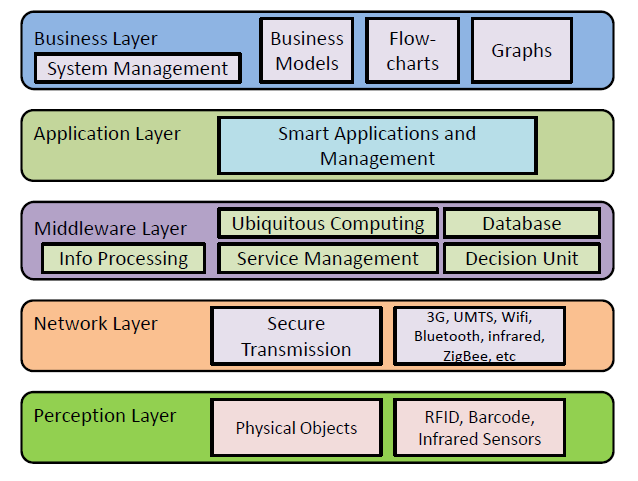
\includegraphics[width=0.8\textwidth]{assets/Abstract_IoT_Architecture.png} 
	\caption{Generic Architecture}
	\label{fig:genericArchitecture}
\end{figure}

\textbf{Perception Layer:} The perception layer or device layer is the layer where physical objects will be able to capture data via sensors. These sensors are able to collect real world data. These data can be or not be processed upstream to add meta-data by the connected object itself and will be forwarded to the Network Layer.

\textbf{Network Layer:} The Network Layer or Transmission Layer. This layer transfers the informations from to Perception Layer to the Middleware Layer. This transfer can be accomplished by different communication technologies like Wifi, 3g, Bluetooth, etc.

\textbf{Middleware Layer:} The Middleware Layer is the common layer for all physical objects of an IoT architecture. The middleware is responsible to take automatic decisions based on informations coming for the devices and store the results in a database. 

\textbf{Application and Business Layer}: The Application Layer is where smart applications are running to produce complex processes. These applications will consume data from connected objects previously processed by the middleware to act effectively on a specific situation. These application can transmit actions to execute on a particular type of service. The Business Layer is important for the global management of the system. This one is rather a layer of global monitoring which produces graphs and statistics at the business level.

\subsection{Data Flow}

The previous architecture can be simplified to highlight the layer of architecture on which this state of the art will focus.
\newline
\begin{figure}[h]
	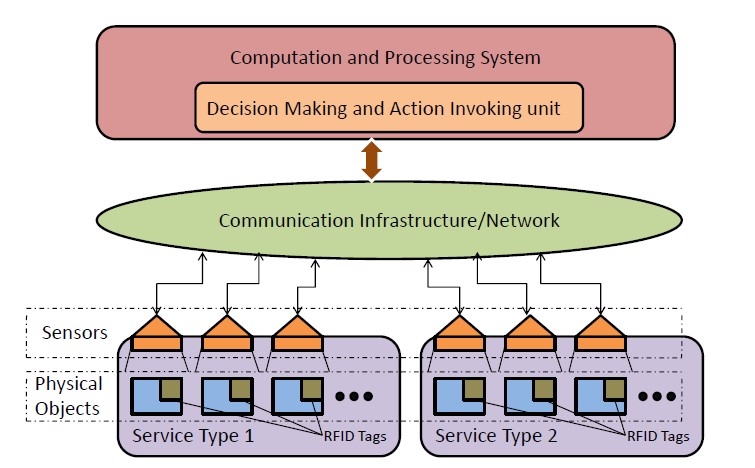
\includegraphics[width=0.8\textwidth]{assets/Basic_IOT_Architecture.png} 
	\caption{Simple IoT Architecture}
	\label{fig:simpleArchitecture}
\end{figure}

This state of the art is focusing on the "Computation and Processing System" layer because at that stage, the data processing is the most critical and the data flow is the highest. Obviously, the Communication Layer must be robust enough to transmit the data efficiently but this topic will not be tackled in this article.

\section{Event Driven Architecture}



\section{Database and Data Stream Management Systems}

Real-time applications are consuming the data in a different way comparing to a traditional system. On a traditional information system using a Database Management Systems (DBMS), the information stored in the database related to an specific entity is a "static" data persisted. The information stored in an aggregation of the reality. Only the current state of the information is relevant for the system. This type of Data management doesn't fit all real-time applications' needs. A real-time application needs to correlate each events coming into the system. An IoT solution is sending too much data into the system. It's not possible for a traditional database to store, query and respond in a timely manner. 
\newline
\newline
The Data Stream Management Systems are designed to handle potentially infinite and fast changing event streams. Obviously, it is not possible to query the all history of events that came from the beginning of the solution and respond in milliseconds. Different approaches exist to limit the amount of data processed. Roughly, compression techniques exists to summarize a set of data already queried. Another technique consists of setting a time window to pick a portion of data in the time. 
%----------------------------------------------------------------------------------------
%	Complex Event Processing
%----------------------------------------------------------------------------------------

\section{Complex Event Processing}

\subsection{Definition}

Complex Event Processing (CEP) is a set of methods and techniques for tracking
and analysing real-time streams of informations and detecting patterns or correlations
of unrelated data (complex events) that are of interest to a particular
business. \cite{1} The complex event processing is the engine of real-time applications that needs to have real-time informations from an environment to respond as fast as possible. A standard Request/Reply with synchronous processes cannot correlate different type of events and respond in a timely manner. Complex Event Processing mechanisms are often used in Event Driven architectures. This architecture fits with the Internet of Things needs. This kind of architecture is driven by events sent by connected objects. Then, the services at the application layer are consuming those events.

\subsection{Event Correlation}

\subsection{CEP Engine}

The CEP engine is consuming the events sent by the physical objects on the Communication Layer. This engine can define a bunch of rules where each event received will be evaluated. A rule represents a complex condition that can be based on multiple events and on a time window. For example, if all connected cameras in a house are sending that there aren't any move in the house in a time window of 60 seconds, an event saying that nobody is in the house will be sent. Then, some specific actions can be taken by connected devices in the house. 
\newline
\begin{figure}[h]
	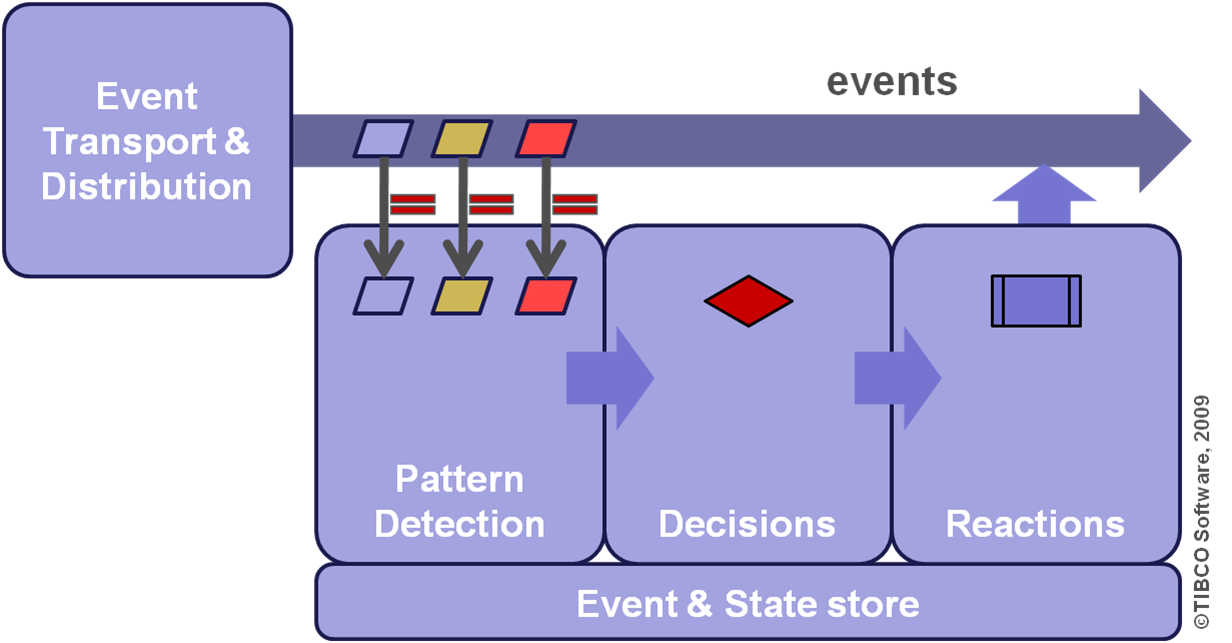
\includegraphics[scale=0.6]{assets/cep-pattern-decision-reaction.png} 
	\caption{CEP Pattern Decision Reaction}
	\label{fig:cep-pattern-decision-reaction}
\end{figure}

The technologies implementing CEP concepts are querying Time Series Databases where each event received are stored. Thoses databases are optimised for queries based on a time window. In a lot of CEP framework like Apache Flink, those CEP rules are describe like an SQL Query and uses Event Pattern Languages. 

\subsection{Event Pattern Languages}

An Event Pattern Language (EPL) is a language used by CEP engines in order to describe the relations between events that match a specific pattern. The syntax of EPL's are quite similar to SQL queries. The Example 1 is retrieving dates where the temperature was bigger than 30 degrees Celsius.
\newline
\newline
\underline{\textbf{Example 1:}}
\begin{verbatim}
	SELECT Thermometer.date
	FROM DataSource
	WHERE temperature > 30
\end{verbatim}
A plenty of primitive operators exists in Event Pattern Languages to describe the rule's behaviour. The following operators are coming from ThingML framework but are available in most of CEP frameworks:
\newline
\newline
\textbf{Selection:} Filters relevant events based on the values of their attributes.\cite{6} For example, we can select all Air Pressure events between 101300 Pa and 101400 Pa.
\newline
\textbf{Projection:} Extracts or transforms a subset of attributes of the events.\cite{6}
\newline
\textbf{Window:} Defines which portions of the input events to be considered for detecting pattern.\cite{6} For example, a rule can concern the last 30 seconds events.
\newline
\textbf{Conjunction:} Consider the occurrences of two or more events.\cite{6} This operator is basically a logical 'AND' operator.
\newline
\textbf{Disjunction:} Consider the occurrences of either one ore more events in a predefined set.\cite{6} This operator is basically a logical 'OR' operator.
\newline
\textbf{Sequence:} Introduces ordering relations among events of a pattern which is satisfied when all the events have been detected in the specified order.\cite{6}
\newline
\textbf{Repetition:} Considers a number of occurrences of a particular event.\cite{6}
\newline
\textbf{Aggregation:} Introduces constraints involving some aggregated attribute values.\cite{6} For example, the average temperature of all Weather events is an aggregation.
\newline
\textbf{Negation:} Prescribes the absence of certain events.\cite{6} This operator is basically a logical 'NOT' operator.

%--------------------------------------------------------------------------------------

\section{Computing Levels}

The main preoccupations of a real-time solution in IoT is to have the lowest latency between all devices. To process all data coming from sensors, CEP engines can help reducing the processing time. The CEP engines can be placed at different level of the IoT architecture. The place where Complex Event Processing is used depends of the business needs. 

%----------------------------------------------------------------------------------------

\subsection{Cloud Computing}

The Cloud Computing places the computing complexity at the cloud level. All the data coming from the sensors have to transit by the connected object, sometimes by a middleware and then it can be consumed by a CEP Engine in the cloud. The Cloud Computing is common for near real-time applications where a little bit of latency is not critical.
\newline
\begin{figure}[h]
	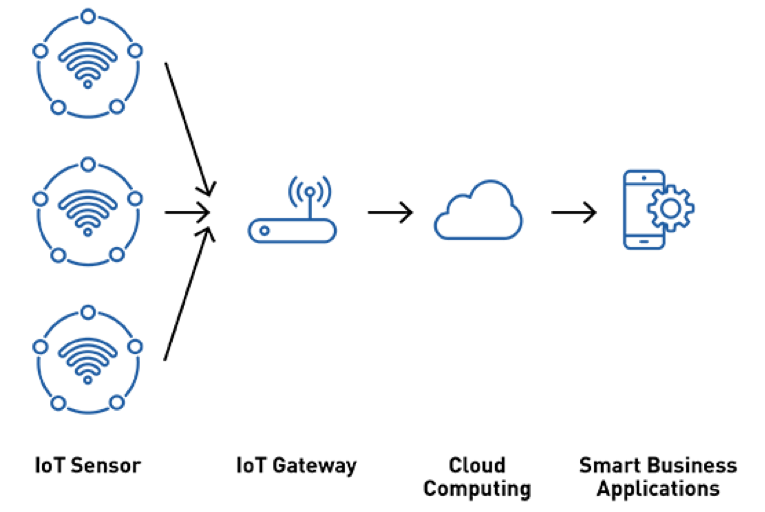
\includegraphics[width=\textwidth,height=160pt]{assets/Cloud_Computing.png}
	\caption{Cloud Computing}
	\label{fig:Cloud-Computing}
\end{figure}

This solution is optimal for the near real-time cloud monitoring because all events coming from the devices are sent to the cloud. Then a precise metrics history can be retrieved. Obviously all data persisted have a cost. This type of solution is extremely demanding in storage space if all the history is persisted.
\newline
\newline
Of course the Cloud Computing can be coupled with other levels of computing and it's often the case. The Cloud Computing can be placed on the top of a multi site IoT solutions where millions of data are coming from thousands of connected objects in the world. Then this solution can reflect a High Level overview of a global IoT system and available all over the world.

%----------------------------------------------------------------------------------------

\subsection{Fog Computing}

The Fog Computing places the computing intelligence at the local network level. Typically the complexity is put between the Cloud and the IoT sensors. The devices are sending their data to a Middleware and the CEP engine is processing the data locally and send the processed events to a service running in the Cloud or on a local server. This method offers the CEP performances on a closer level where the data are created. Then the applications where latency is crucial, the Fog Computing can fit with their business needs. For example, the auto mobile or aerospace sector are more and more connected and the reactivity of their system needs to be as fast as possible.
\newline
\begin{figure}[H]
	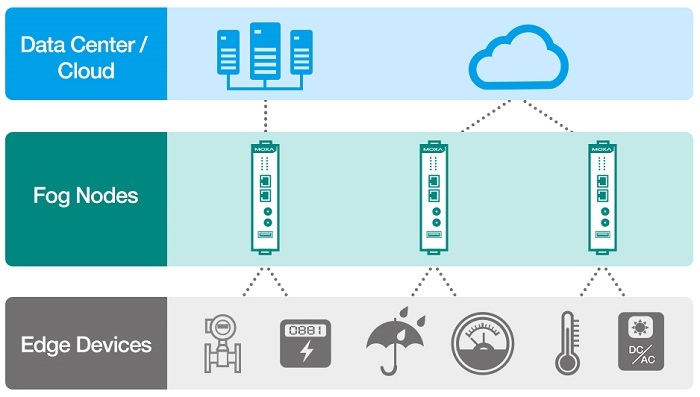
\includegraphics[width=\textwidth,height=160pt]{assets/Fog_Computing.jpg}
	\caption{Fog Computing}
	\label{fig:Fog-Computing}
\end{figure}

It can happen that the edge devices are sending too much data and very fast. Then the fog computing can still respond too slowly because of the massive data reception. The CEP philosophy can be put at the lowest level with Edge Computing.

%----------------------------------------------------------------------------------------

\subsection{Edge Computing}

Edge computing refers to the enabling technologies allowing computation to be performed at the edge of the network,on downstream data on behalf of cloud services and upstream data on behalf of IoT services. Here we define “edge” as any computing and network resources along the path between data sources and cloud data centers.\cite{Edge Computing - Vision and Challenges}
\newline\newline
The Edge Computing places the computing complexity at the Physical Layer. This method reduces the network traffic to the Fog Nodes and the Cloud because less informations will be transferred. Therefore it reduces the risk of data congestion and the CEP engines are not flooded. Edge Computing is generally used by industries in Cyber Physical Systems\footnote{Cyber-Physical Systems (CPS) are integrations of computation and physical processes. Embedded computers and networks monitor and control the physical processes, usually with feedback loops where physical processes affect computations and vice versa \cite{5}}.

%----------------------------------------------------------------------------------------

\section{Semantic Complex Event Processing}

The publish-subscribe pattern in software architecture is a messaging pattern where the sender of the message doesn't know the receiver. On the other side, the receiver doesn't know the sender as well. The publisher is sending a message on a message queue where subscriber(s) are listening to. In Internet of Things solutions, the producers and consumers can be the connected objects themselves but it can also be an application layer in the Cloud for example. The connected objects are publishing events on event topics and the application layer processes those events. They process those events with CEP engines and when the pattern is matching with a defined rule, they send messages to the connected objects through message queues. Then, the connected objects can update their state and perform actions.
\newline
\newline
The article "A Semantic Publish-Subscribe Architecture" \cite{A Semantic Publish-Subscribe Architecture} suggests an interesting asynchronous architecture based on the Publish-Subscribe design pattern. This architecture prone the modularity, extensibility and cost-effective vision. It splits the physical world from its digital representation. The primary characteristic consists of splitting clients into 3 categories: consumers, producers and aggregators. The business logic is driven by the aggregators. The producers and the consumers are the bridge between the physical world and the virtual representation of the systems. This principle keeps the business logic at the aggregator level in order to keep the clients and producers as simple as possible. It gives to the producers the unique responsibility to send data to an upper layer without executing any business logic. Hence, this system is easier to extend because only the aggregator layer is impacted if a business feature is added. Then, the consumers and producers can be shared by different applications.
\newline
\newline
The role of the producers is to collect the data from the sensors. The producer can optionally make a local processing where it encapsulate the data to a semantic format. After that, the producer send the information to the SUB Engine where a CEP Engine will process the event.
Contrarily, the consumers are listening to the concrete events coming in the SUB Engine that can be a result of a Complex Event Processing from a CEP Engine and/or a process done by an Aggregator. After receiving an notification, the consumers extract the raw data and send it to a devices through a legacy interface.

\section{Micro-services Architecture}

\section{Penser à parler de tous les termes (raw event, simple event, complex event, Event Processing Agent...)}

%----------------------------------------------------------------------------------------

\section{IoT Platform extension}


%----------------------------------------------------------------------------------------

\section{Problematic}

%----------------------------------------------------------------------------------------

\section{Research Methodology}

%----------------------------------------------------------------------------------------

\section{Conclusions}

%----------------------------------------------------------------------------------------
%----------------------------------------THE END-----------------------------------------
%----------------------------------------------------------------------------------------

\newpage
\listoffigures
\nocite{*}
\printbibliography

\end{document}
